\comment{Suggestion: past tense}\\

\subsection{Gradient Descent Analysis}
    
    \subsubsection{OLS Optimisation}
        All plots regarding the optimisation of the OLS cost function are found in \cref{res:fig:lrates}. The best MSE scores and learning rates are tabulated in \cref{res:tab:OLS_MSEs}. We found that the none of the algorithms come really close to the analytical OLS solution, found by matrix inversion, with a validation MSE of $0.1176$. The best performing algorithms were SGD with Adam (MSE $0.1736 \pm 0.0016$), SGD with momentum (MSE $0.1754 \pm 0.0023$) and SGD with AdaGrad and momentum (MSE $0.1762 \pm 0.0028$).

        In \cref{res:fig:lrate1} we see that the non-stochastic GD algorithm performed well when momentum was added, giving it a chance to avoid any local minima. However, the stochastic methods converged faster, and especially when momentum is added, converged well for a large range of learning rates (from around 0.02 to 0.1).

        Exploring the increase in epochs and decrease in batch size in \cref{res:fig:lrate2}, we see that decreasing batch size made the algorithm less stable, and more easily prone to exploding gradients. Increasing the number of epochs improved the result much the same as decreasing batch size, but decreased stability, just not as much as decreased batch size.



        \comment{Reminder: Mention AdaGrad SGD not converging within range.-\Carl}
        \begin{table}[!ht]
            \centering
            \begin{tabular}{r|c|l}
                Method & MSE & $\eta$ \\ \hline
                Plain GD & $0.327 \pm 0.056$ & 0.072 \\
                Momentum GD & $0.1843 \pm 0.0057$ & 0.13 \\
                Plain SGD & $0.1948 \pm 0.0070$ & 0.065 \\
                Momentum SGD & $0.1754 \pm 0.0023$ & 0.040 \\
                AdaGrad GD & $0.369 \pm 0.074$ & 0.43 \\
                AdaGrad Momentum GD & $0.234 \pm 0.019$ & 0.49 \\
                AdaGrad SGD & $0.2031 \pm 0.0092$ & 0.70 \\
                AdaGrad Momentum SGD & $0.1762 \pm 0.0028$ & 0.30 \\
                RMSprop SGD & $0.1933 \pm 0.0060$ & 0.036 \\
                Adam SGD & $0.1733 \pm 0.0016$& 0.092 \\
            \end{tabular}
            \caption{Table of the best validation MSE scores by GD algorithm, together with the learning rate that produced the best result.}
            \label[tab]{res:tab:OLS_MSEs}
        \end{table}

        \begin{figure*}
            \begin{subfigure}{.49\textwidth}
                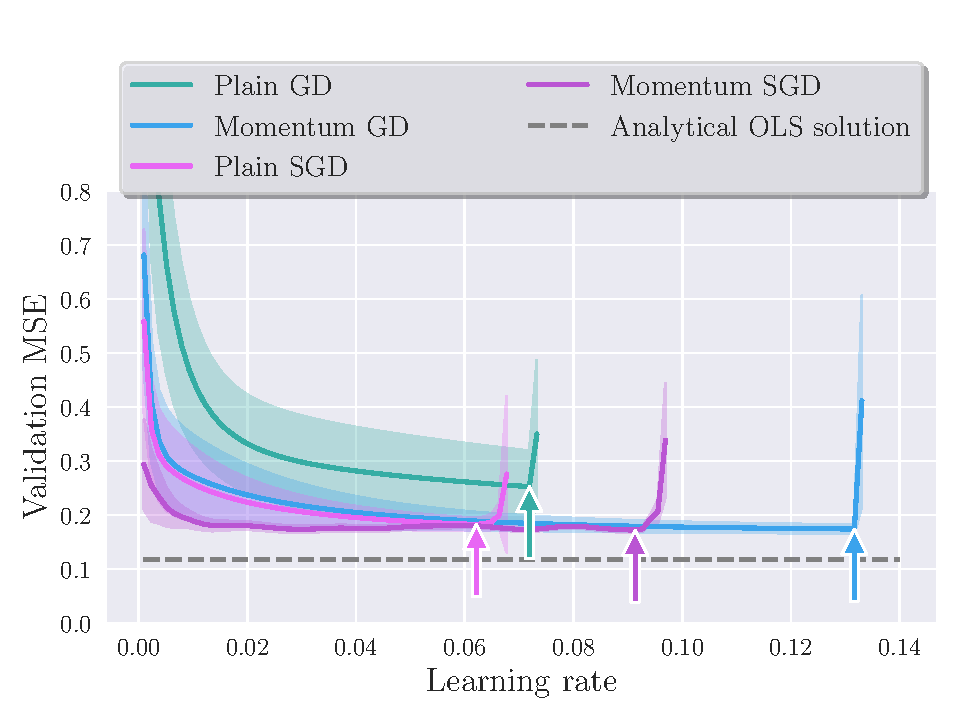
\includegraphics[width=\linewidth]{learning_rates_PGD_MGD_PSGD_MSGD.pdf}
                \caption{The minimal MSEs by algorithm: plain GD 0.327 ($\eta=0.072$), GD w/ momentum 0.1843 ($\eta=0.13$), plain SGD 0.1948 ($\eta=0.065$), SGD w/ momentum 0.1754 ($\eta=0.040$)}
                \label[fig]{res:fig:lrate1}
            \end{subfigure}
            \hfill
            \begin{subfigure}{.49\textwidth}
                \centering
                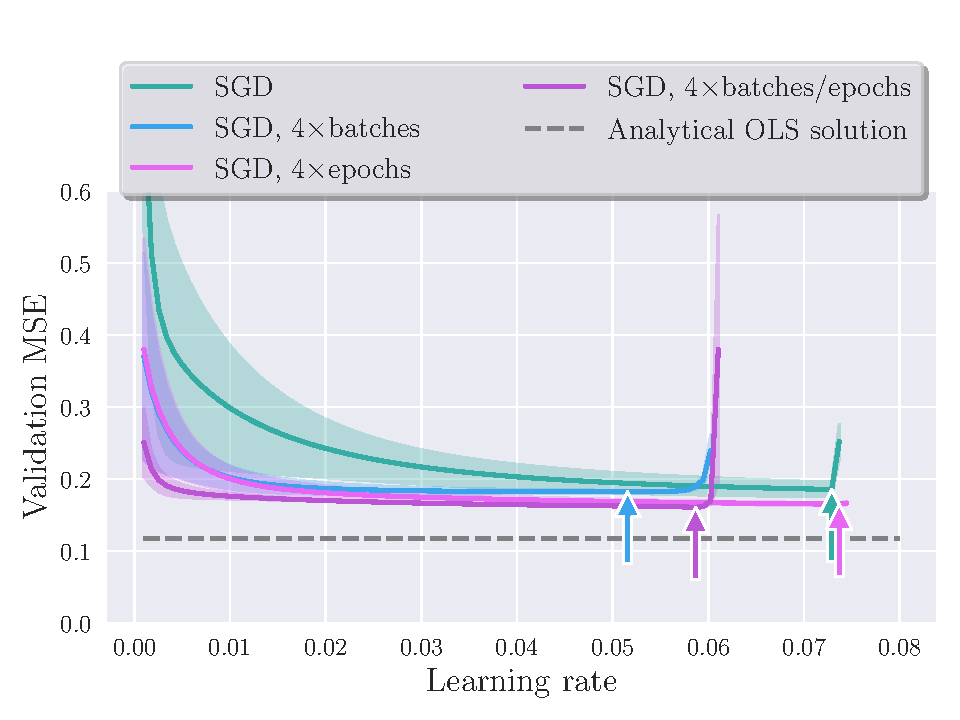
\includegraphics[width=\linewidth]{learning_rates_SGD_batches_epochs.pdf}
                \caption{The minimal MSEs of plain SGD by number of epochs and batch size: 100 epochs/64 batch size 0.1948 ($\eta=0.065$), 100 epochs/16 batch size 0.1836 ($\eta=0.032$), 400 epochs/64 batch size 0.1743 ($\eta=0.046$), 400 epochs/64 batch size 0.1797 ($\eta=0.0028$)}
                \label[fig]{res:fig:lrate2}
            \end{subfigure}
            \hfill
            \begin{subfigure}{.49\textwidth}
                \centering
                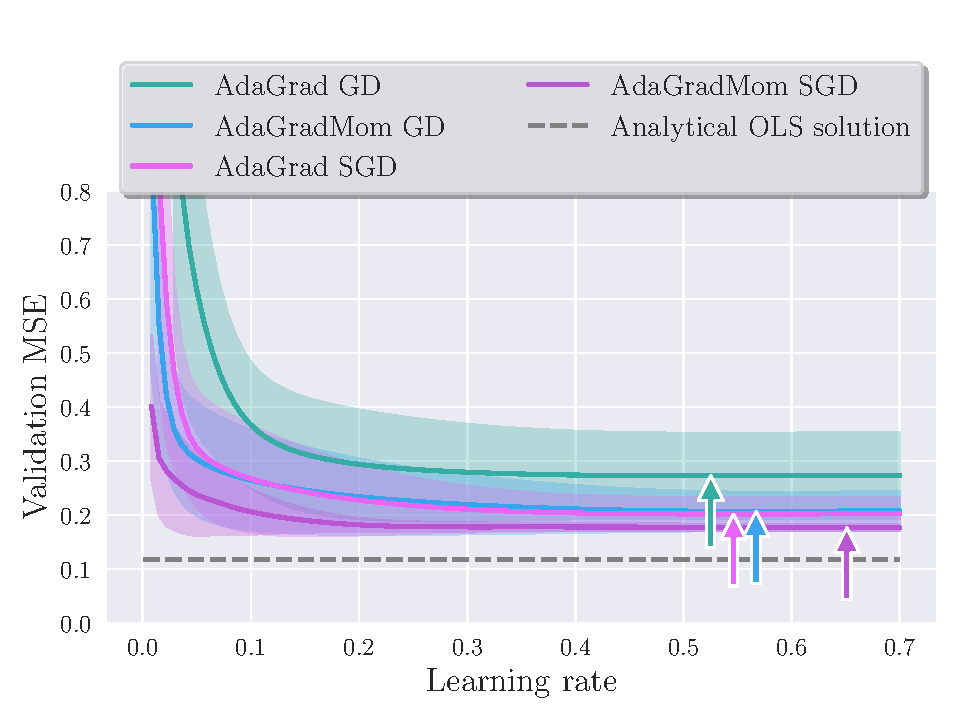
\includegraphics[width=\linewidth]{learning_rates_adagrad}
                \caption{The minimal MSEs by algorithm: AdaGrad GD 0.3688 ($\eta=0.074$), AdaGrad GD w/ momentum 0.2345 ($\eta=0.49$), AdaGrad SGD 0.2031 ($\eta=0.70$), AdaGrad SGD w/ momentum 0.1762 ($\eta=0.30$)}
                \label[fig]{res:fig:lrate3}
            \end{subfigure}
            \hfill
            \begin{subfigure}{.49\textwidth}
                \centering
                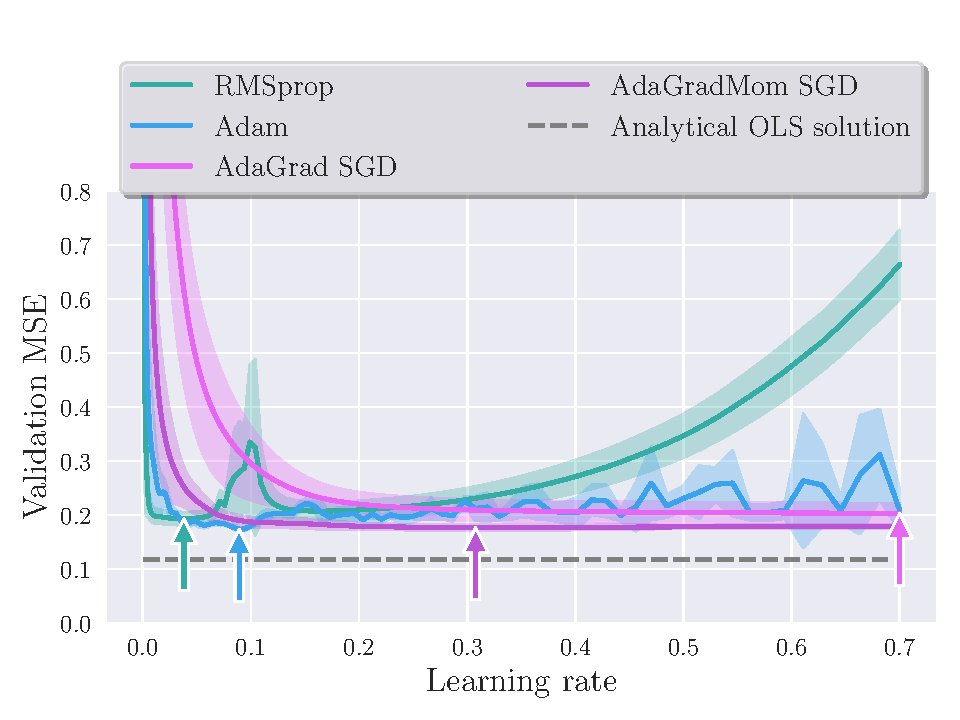
\includegraphics[width=\linewidth]{learning_rates_tunable}
                \caption{The minimal MSEs by algorithm: RMSprop SGD 0.1933 ($\eta=0.036$), Adam SGD 0.1733 ($\eta=0.092$), AdaGrad SGD 0.2031 ($\eta=0.70$), AdaGrad SGD w/ momentum 0.1762 ($\eta=0.30$)}
                \label[fig]{res:fig:lrate4}
            \end{subfigure}
            \caption{Plots of the validation MSE of the parameters found from optimising the OLS cost function on Franke function data with $n=600$ data points. For the momentum methods we used $\gamma=0.8$, for RMSprop we used $\beta=0.9$ and for Adam we used $\beta_1=0.9, \beta_2=0.99$. The stochastic methods used a batch size of 64 and 100 epochs, while the standard GD did 100 iterations unless specified otherwise. Overlaid are 95\% confidence intervals based on optimising with five different starting points.
            Analytical OLS MSE: 0.1176.}
            \label[fig]{res:fig:lrates}
        \end{figure*}

    \subsubsection{Ridge Optimisation}
        The results from the ridge analysis are found in \cref{res:fig:GDridge}. 

        \begin{figure*}
            \begin{subfigure}{.49\textwidth}
                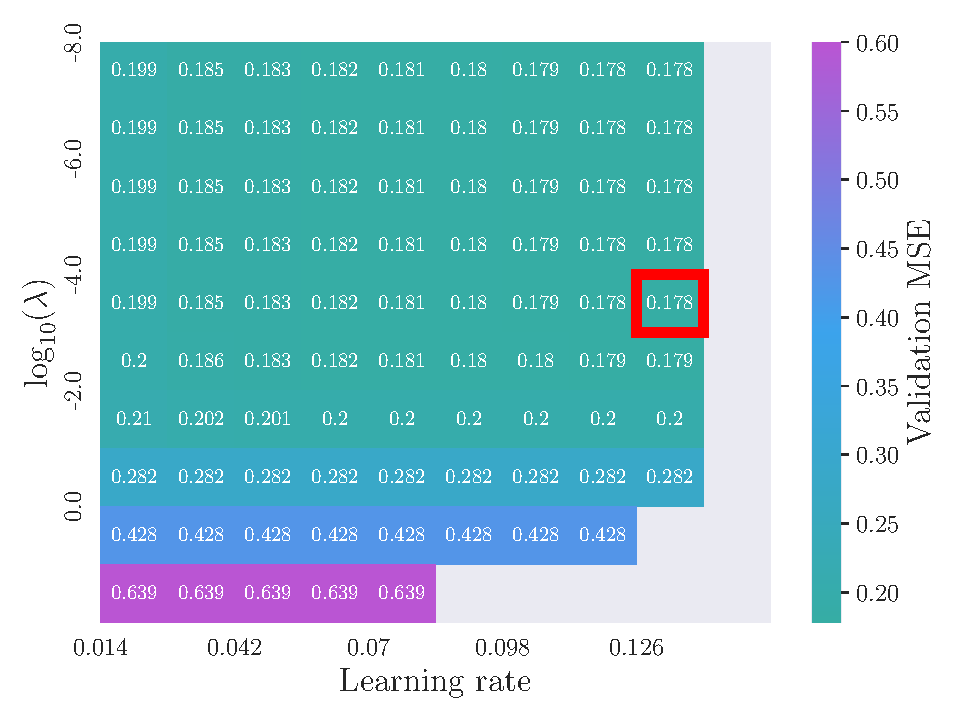
\includegraphics[width=\linewidth]{lmbda_learning_rates_momentum_GD.pdf}
                \caption{\textbf{GD with momentum}. Best MSE value was 0.1843 with $\lambda=0.0032, \eta=0.13$.}
                \label[fig]{res:fig:mGDridge}
            \end{subfigure}
            \hfill
            \begin{subfigure}{.49\textwidth}
                \centering
                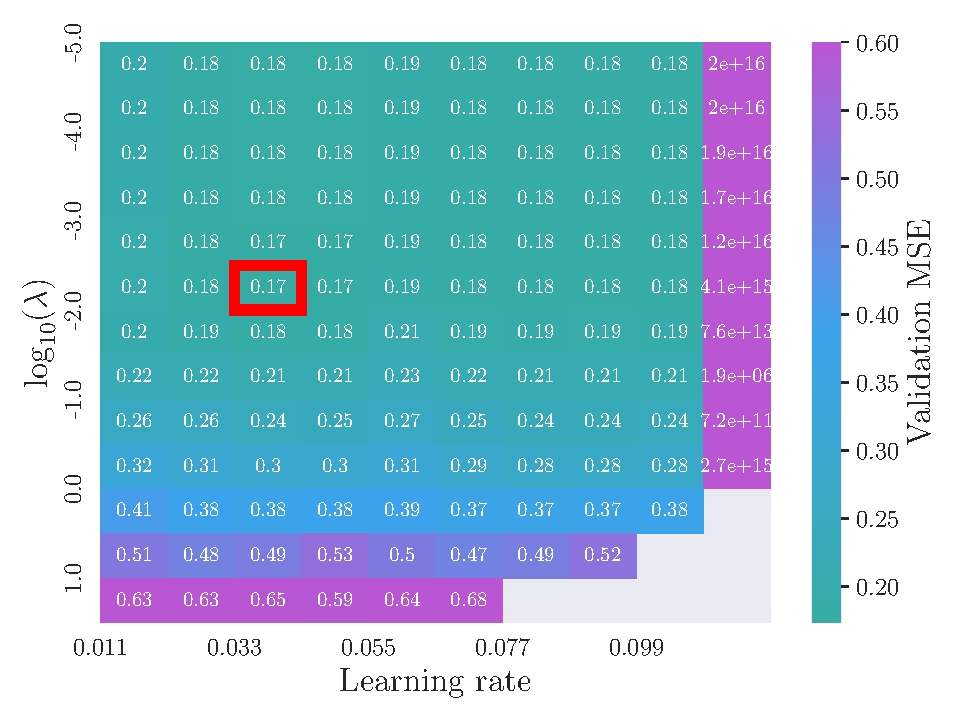
\includegraphics[width=\linewidth]{lmbda_learning_rates_momentum_SGD.pdf}
                \caption{\textbf{SGD with momentum}. Best MSE value was 0.1734 with $\lambda=0.0032, \eta=0.033$.}
                \label[fig]{res:fig:mSGDridge}
            \end{subfigure}
            \hfill
            \begin{subfigure}{.49\textwidth}
                \centering
                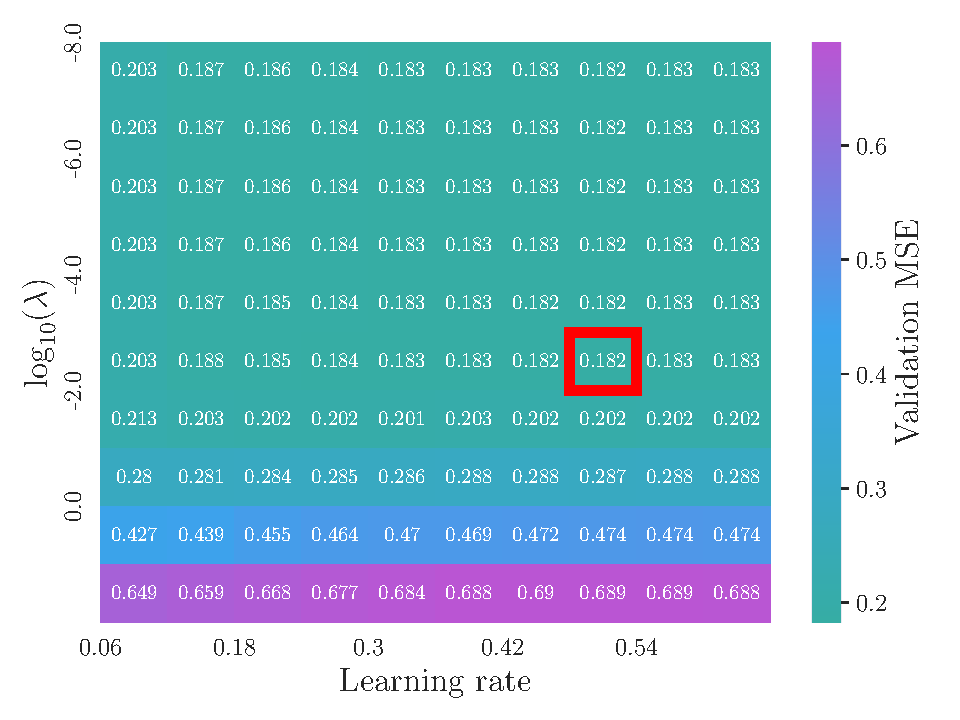
\includegraphics[width=\linewidth]{lmbda_learning_rates_adagrad_momentum_SGD.pdf}
                \caption{\textbf{SGD AdaGrad with momentum}. Best MSE value was 0.1745 with $\lambda=0.0032, \eta=0.30$.}
                \label[fig]{res:fig:agSGDridge}
            \end{subfigure}
            \hfill
            \begin{subfigure}{.49\textwidth}
                \centering
                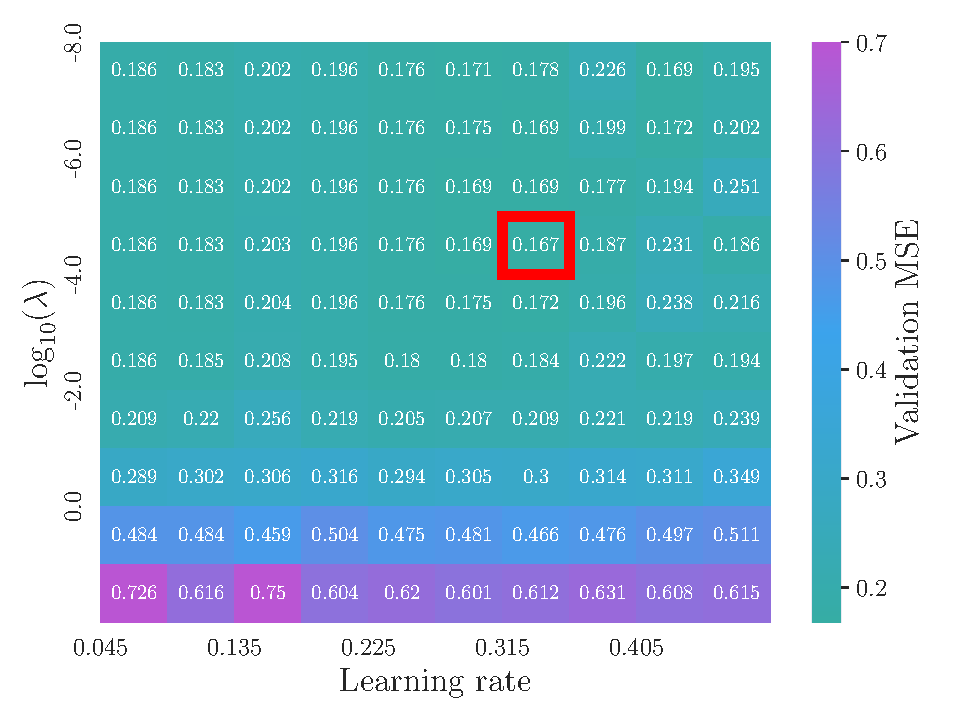
\includegraphics[width=\linewidth]{lmbda_learning_rates_adam_SGD.pdf}
                \caption{\textbf{SGD Adam}. Best MSE value was 0.1724 with $\lambda=0.0010, \eta=0.090$.}
                \label[fig]{res:fig:adSGDridge}
            \end{subfigure}
            \caption{}
            \label[fig]{res:fig:GDridge}
        \end{figure*}


\subsection{Wisconsin Breast Cancer}
    \begin{figure*}
        \begin{subfigure}{.49\textwidth}
            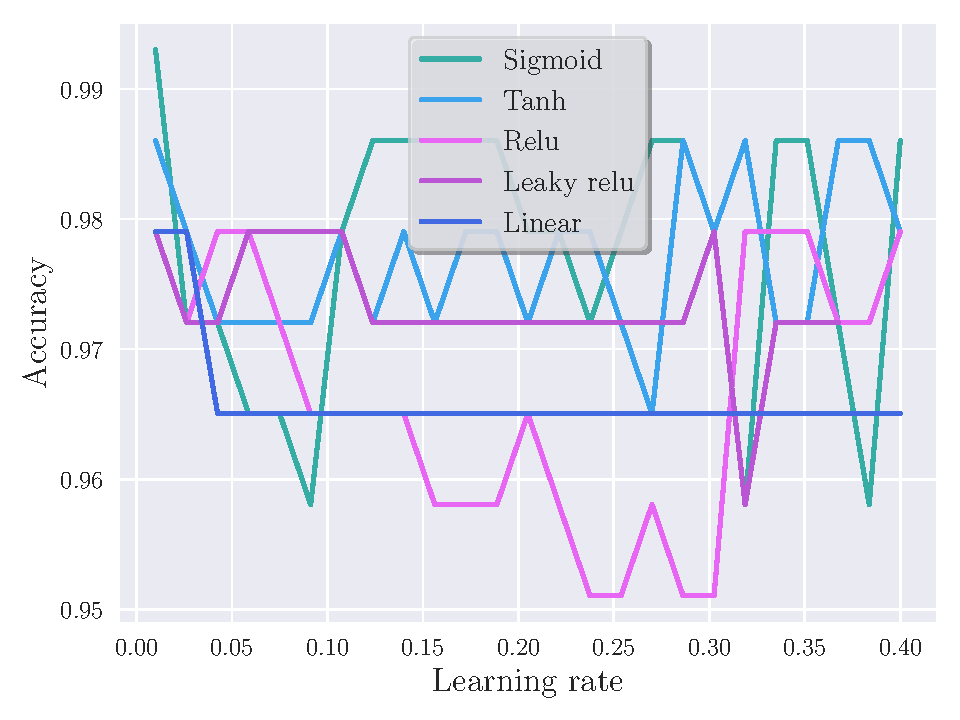
\includegraphics[width=\linewidth]{clasf_activation_functions1.pdf}
            \caption{$\eta \in [ 0.01, 0.4 ]$ with $n = 50$ points. One hidden layer with a single node}
            \label[fig]{res:fig:a}
        \end{subfigure}
        \hfill 
        \begin{subfigure}{.49\textwidth}
            \centering
            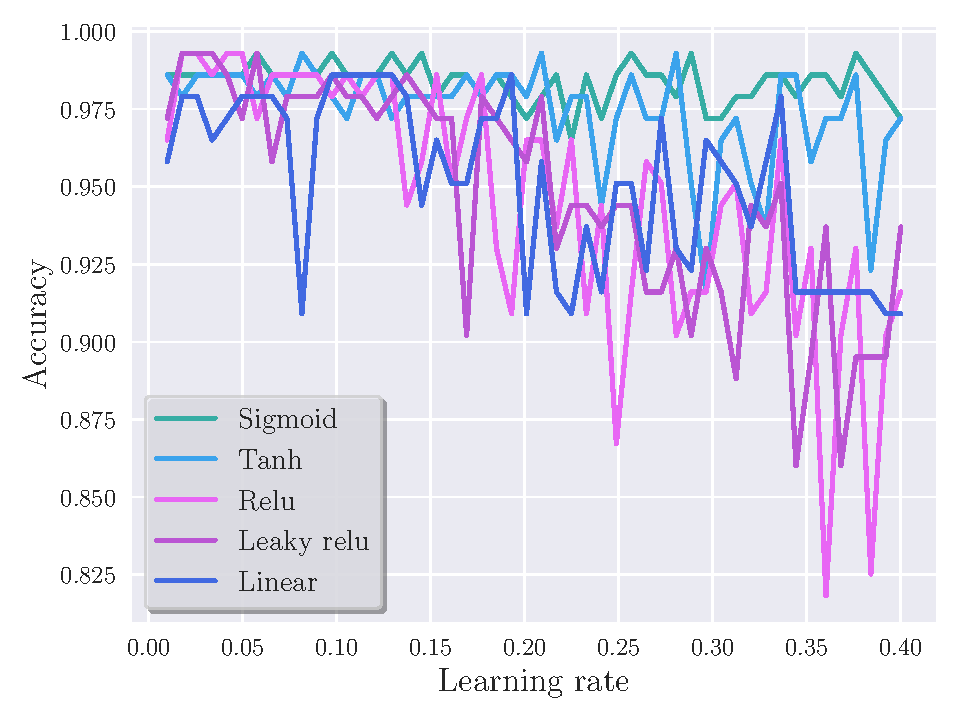
\includegraphics[width=\linewidth]{clasf_activation_functions2.pdf}
            \caption{$\eta \in [ 0.001, 0.01 ]$ with $n = 50$ points. One hidden layer 30 nodes}
            \label[fig]{res:fig:b}
        \end{subfigure}
        \hfill 
        \begin{subfigure}{.49\textwidth}
            \centering
            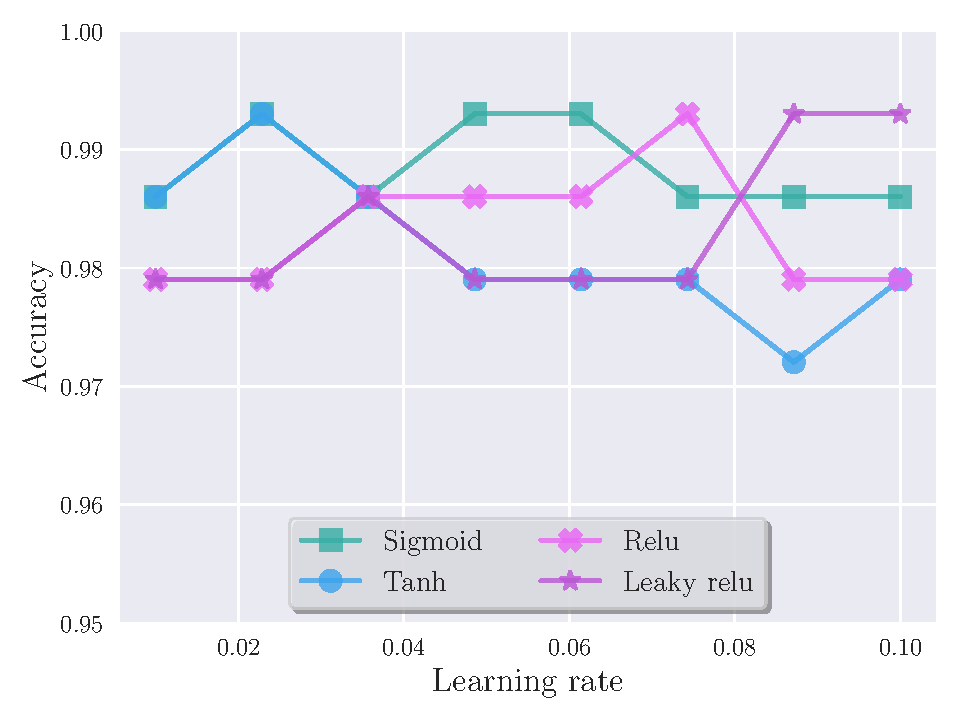
\includegraphics[width=\linewidth]{clasf_activation_functions3.pdf}
            \caption{$\eta \in [ 0.001, 0.01 ]$ with $n = 50$ points. Two hidden layers with 15 nodes each}
            \label[fig]{res:fig:c}
        \end{subfigure}
        \hfill 
        \begin{subfigure}{.49\textwidth}
            \centering
            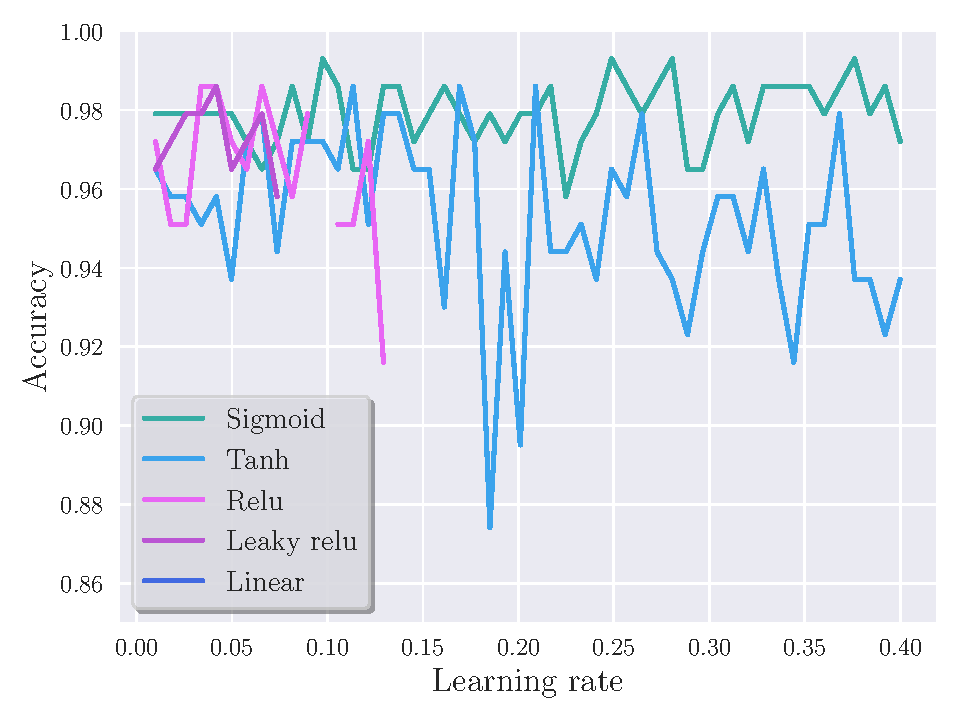
\includegraphics[width=\linewidth]{clasf_activation_functions4.pdf}
            \caption{$\eta \in [ 0.001, 0.01 ]$ with $n = 50$ points. Three hidden layers with ten nodes each}
            \label[fig]{res:fig:d}
        \end{subfigure}
    \end{figure*}